\documentclass{article}
\usepackage{graphicx}
\usepackage{float}

\graphicspath{ {images/} }

\newcommand{\projectnaam}{Software Reengineering}
\newcommand{\student}{Van Muylder Ben \& Geeraert Lander}
\title{\textmd{\textbf{Final Project Report}}\\\normalsize\vspace{0.1in}\Large{\projectnaam}}
\author{\student}\date{\today}

\setcounter{section}{-1}

\begin{document}
\maketitle
\newpage

\section{Introduction}

The purpose of this project is to plan a refactoring for an existing software project such that we can easily add newly requested features.
The exiting software for this project is JFreeChart, and the functionality which we wish to add is the possibility to (1) have a plot where each data point is a different shape and (2) have the ability to read all different shapes from a database.\\

To be clear, we are not meant to implement these features, rather we are to refactor the project such that it would be easy for a developper to add these features.

\section{General Plan}

We will start by informing ourselves of the current structure and workings of this library. More specifically, we will figure out where and how exactly plots are generated in the code.\\

Using CodeScene, we looked at which classes it suggested needed refactoring (classes which were hotspots). This lead us to the XYPlot Class, which effectively is the class which renders plots.\\

XYPlot then uses a XYItemRenderer, or rather a class which implements the XYItemRenderer interface to effectively render its plots. Such a class could be XYLineAndShapeRenderer, which effectively renders a plot with shapes and lines which connects these shapes.\\

However, a XYLineAdnShapeRenderer is not capable of rendering a data set with all different shapes (which is were the assignment comes in place).\\

As such we can note that the ability for a serie of a plot to have a shape is already present it the code. This specific part is contained in the AbstractRenderer class. However, the class only allows you to set one specific shape for a serie. This is where we presume that our initial refactoring will take place.\\

For now we plan to split up the shape setting code/function to allow more flexible shape setting, for example: using multiple functions such as SetSeriesShapeUnique, SetSeriesShapeByType (where the type could be random)...

\begin{figure}[H]
\centering
	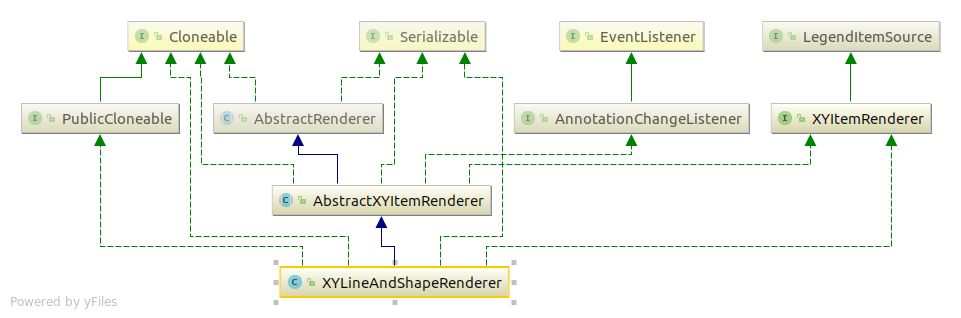
\includegraphics[width=0.9\textwidth]{XYLineAndShapeRenderer.png}
	\caption{an overview of the XYLineAndShapeRenderer and its dependencies}
\end{figure}

\section{The Refactoring Process}

\subsection[Section Title. Section Subtitle]{Refactoring Stage 1\\ {\large Extracting the shape functionality}}


\subsubsection{Analysis}

As we discussed in the plan, we had found that the functionality which assigns the effective icon to a point on the plot resides in the AbstractRenderer class, more specifically in the function SetSeriesShape. We also discussed that we thought the initial refactor would be doen around this function. In this subsection, we'll discuss that refactor in further detail.\\

Let us first talk about what functionality this class, AbstractRenderer, already has concerning shapes. Among many other properties, the class has a defaultShape, a shapeList (which are both private properties) and a DEFAULT\_SHAPE (which is public, but only exists to set the initial value for the private defaultShape in the constructor of AbstractRenderer). There is also a property autoPopulateSeriesShape.\\

shapeList is a list which holds a shape for each serie from the renderer.
This means we can get 'get' (and 'set') the shape of each seperate serie. If the autoPopulateSeriesShape property should be true, and a series does not yet have an assigned shape, the 'get' function will try to assign a shape using a DrawingSupplier. We might further elaborate what this class is and does later on in the report, but it serves no further relevance here (as it supposed function seems clear from the class name). If the property autoPopulateSeriesShape should not be true, the serie shall remain without shape, but the default shape (defaultShape) will be returned.\\ 

From above mentioned behavior we can see that only a whole serie can have a shape (as opposed to single points from a serie). This is a logical choice, since we often generate series on plots not knowing how many points effectively will be generated, let alone that we would assign a different shape to those points. However, this current implementation does not allow for the requested behavior (as we have mentioned before).\\

Another general thing to note is that this class (AbstractRenderer) has a lot of functionality. We're not saying that this class is a god class, but we're also not saying that it's not a god class. Because of this it might be a good idea to consider splitting up some of the functionality of the class, particularly: the parts which are interesting for our case (functionality concerning shapes).

\subsubsection{Plan \& Execution}

As we mentioned above, the AbstractRenderer class contains a lot of functionality, and that it might be a good plan to split up some of that functionality. That is what we plan to do to allow for the requested behaviour to be easily implemented. The plan is to take away the current functionality concerning shapes from the class, to put that functionality inside a separate class, which then will be used (or extended) by the AbstractRenderer class.\\ 

Having the original (and possibly slightly changed) functionality in a separate class, will allow future developpers to easily implement new features regarding the original functionality (in our case; shapes).

\begin{figure}[H]
\centering
	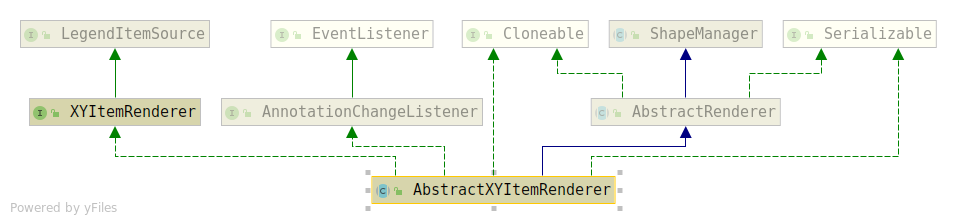
\includegraphics[width=0.9\textwidth]{RefactorStage1aDesign.png}
	\caption{an overview of the AbstractXYItemRenderer and its dependencies, in respect to our proposed design change}
\end{figure}

To be able to pull away the current functionality from the AbstractRenderer class, we have to know if this won't cause any implications on other parts of the code. We know that AbstractRenderer (indirectly) implements parts of XYItemRenderer, so it's possible that other classes might implements those parts of XYItemRenderer in another way. We'll use the 'find implementation(s)' feature of IntelliJ; which only directed us to the implementations from AbstractRenderer.

Because of this we know we can safely pull away the shape functionality from the AbstractRenderer class, as long as AbstractRenderder then extends the class which has the functionality. \\

\noindent
Now, the strange relation that exists between XYItemRenderer and AbstractXYItemRenderer also exists between CategoryItemRenderer and AbstractCategoryItemRenderer. It's important to note this since AbstractXYItemRenderer (and those classes which inherit from it) are not the only ones affected by the creation of the ShapeManager class.

\begin{figure}[H]
\centering
	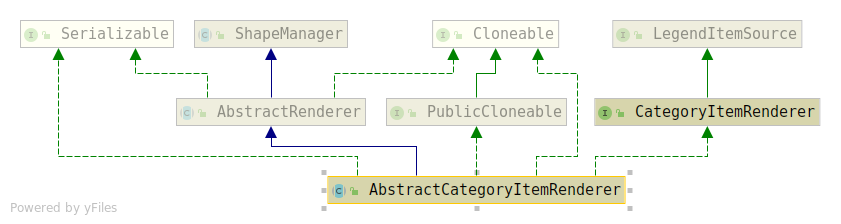
\includegraphics[width=0.9\textwidth]{RefactorStage1bDesign.png}
	\caption{an overview of the AbstractCategoryItemRenderer and its dependencies, in respect to our proposed design change}
\end{figure}

\subsubsection{Intermediate Conclusion}

To be clear: the above mentioned refactor is done to offer some more clarity in finding the right place to add implementation. Too be able to have singular plot points have their own, new functionality will have to be added in the renderers. For this reason we pulled away the current functionality for shapes, and put it in a separate class. For future additions to the project (as mentioned in the project assignment), location the relevant pieces of existing functionality will be a lot simpler and faster.\\

Other functionality could also be pulled away into separate classes, but that would be out of scope for this project.

\subsection[Section Title. Section Subtitle]{Refactoring Stage 2\\ {\large Understanding the shape functionality}}

\subsubsection{Analysis}

To better understand why we pulled away the shape implementation from AbstractRenderer into its own separate class, we'll need to have a further understanding of how and why this functionality is (and isn't) used.

We'll be honest and upfront in saying that we won't have a whole explanation of how this library works, but rather a simplified view of happens in general (with possible deeper insights in those aspects which need more explanation).\\

A shape can be used for many things, but with respect to the assignment; it's used to represent a datapoint on a plot. A datapoint can be a point of its own, or it can be part of a set of datapoints (which we mostly refer to as a serie). This serie might represent a lot of things such as just simply random points, points of data which have been imported, points which represent a (mathematical) function... 

However, purely in data, a shape has not much meaning. The shape itself is meant so we, the user of the library, can see these points on a screen. And when does this happen? When we export our plot (and data) to an image for example.\\

This is where our overview of the workings begin. When we want to export to an image, we'll want to output some data to a buffer. The output comes from a draw function which is a central part of the core functionality, which in itself calls the draw functionality of the Plot interface (which is implemented by XYPlot and CategoryPlot among others...). These draw funtions do a lot of things, but one thing in particular: they render data items, or at least, set this process into motion. XYPlot for example has its own render function, which then in itself calls to the drawItem function of the renderer for that class instance (which would be an XYItemRenderer, which is in itself an interface, but is implemented in a lot of derived classes such as XYLineAndShapeRenderer). The drawItem functionality of XYLineAndShapeRender works with different passes: a first pass which draws the background, and a second pass which draws effective data items.\\

We have now reached the point where we will effectively interact with our ShapeManager. Since XYLineAndShapeRenderer extend AbstractXYItemRenderer, which extends AbstractRenderer, which extends ShapeManager, we can now access the functionality which had been pulled away from AbstractRenderer. The second render pass will get the shape for a specific data item (which will be the same shape for all other data items of that serie) by calling getItemShape.\\

getItemShape is special in 2 ways. The first way is in that it will always return the same shape for data items of the same serie (because of the deeper implementation of this function). The second way is that it is called in many other classes which are extensions of AbstractXYItemRenderer and AbstractCategoryItemRenderer; unlike the function setSeriesShape (and setItemShape, which is a function which doesn't exist (yet)).\\

The function to set a specific shape for a serie, is never used in the whole project. But plots still need shapes for their data points? This is where default shapes come in play. Classes can set a default shape by either changing the value for the default shape in the constructor, or by setting a shape for the series legend and then later on requesting the shape of the data point via the shape of the legend of that serie. 



\newpage
\section{Conclusion}


\end{document}